\documentclass[./\jobname.tex]{subfiles}
\begin{document}
%
%
\chapter{Projektbeschreibung}
%
In diesem Projekt ist Herr Prof. (FH) Dipl.-Ing. Horatiu Pilsan der Auftraggeber. Der Auftraggeber stellt als Aufgabe, eine Software für ein virtuelles Förderband mit dem vorhanden Laboraufbau zu erstellen. Der DC-Motor fungiert hierbei als Simulation des Förderbandantriebes. Die Förderbänder können entweder lokal betrieben (\modeA) oder zusammengeschlossen werden, um eine geschlossene Kette einzurichten (\modeB). Der Zweck ist, virtuelle \paket{e} mit dieser Kette zu transportieren. Es gibt im gesamten fünf virtuelle Förderbänder, die als Ring zusammengeschlossen werden können.
%
\section{Laboraufbau}
%
Für die Simulation wird ein Laboraufbau verwendet, der ein Förderband praxisnah simuliert. Dieser Aufbau beinhaltet die folgenden Komponenten:
%
\begin{itemize}
\item Mikrocontrollerboard mit VxWorks v6.9 als Betriebssystem
\item DC-Motor als Förderbandantrieb
\item Display und Keyboard für das User Interface
\item 2 Netzwerkverbindung
%\item PT100 Temperatursensor zur Überwachung der Motortemperatur
\end{itemize}
%
In den folgenden Abschnitten erfolgt eine kurze Beschreibung der zu realisierenden Betriebsarten \modeA und \modeB.
%
\section{\modeA}
%
Der \modeA, der Service-Betriebsmodus, ist für Situationen vorgesehen, wo ein manuelles Eingreifen benötigt wird. Es muss möglich sein, das Profil wie in \autoref{fig: motor-geschwindigkeitsprofil.pdf} dargestellt in beide Richtungen zu starten. Vor dem Start des Profils kann die Geschwindigkeit in einem definierten Bereich geändert werden.
% im Bereich von \minMaxVelocity in Schritten von \stepSizeMotor zu ändern. 
Die Bedienung des Förderbandes erfolgt über die Tastatur oder über eine \gls{telnet} Verbindung. 
%Das Profil ist in \autoref{fig: motor-geschwindigkeitsprofil.pdf} abgebildet.
%
\begin{figure}[H]
	\centering
	\noindent\adjustbox{max width=\textwidth}{%falls größer als \textwidth, wird das Bild verkleinert
		%trim option's parameter order: left bottom right top
		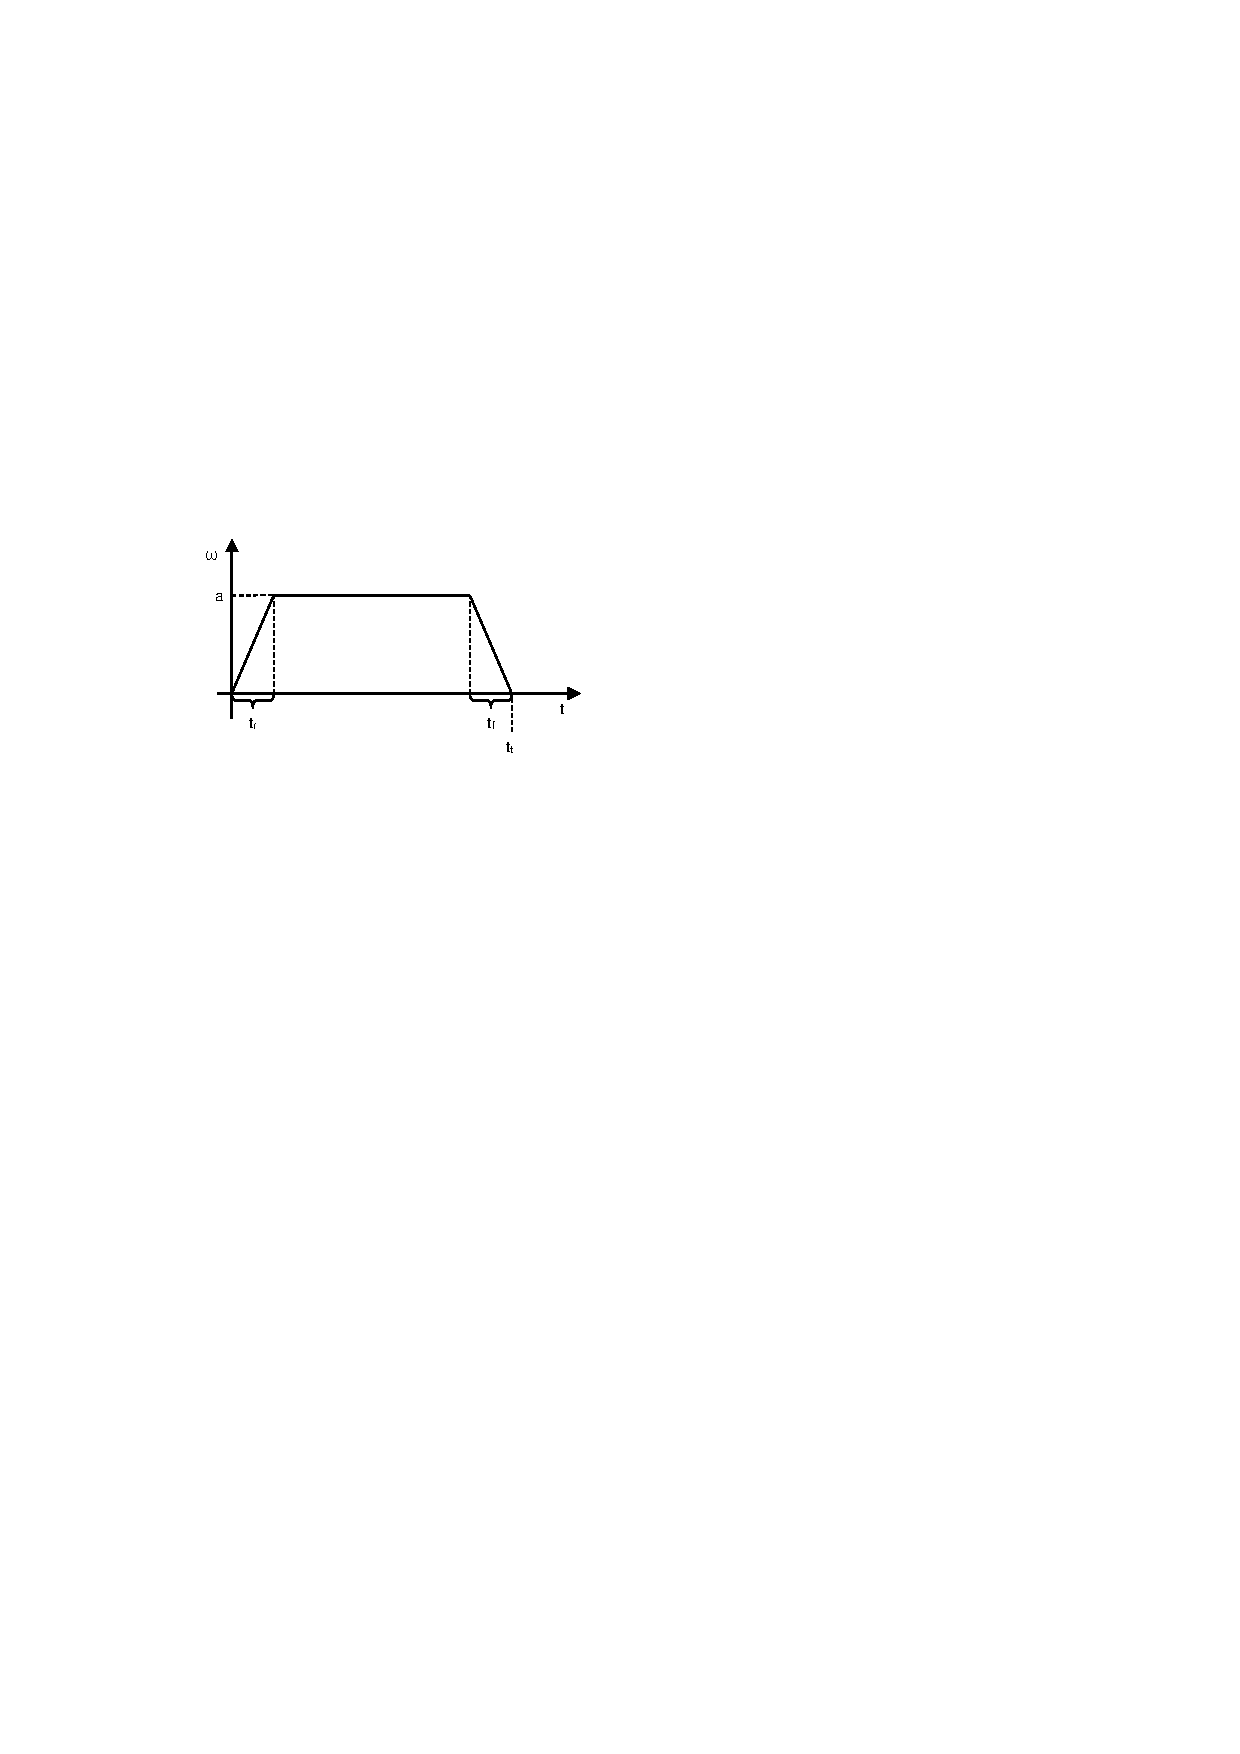
\includegraphics[width=0.6\textwidth]{./img/0_Projektbeschreibung/motor-geschwindigkeitsprofil.pdf}
	}
	\unterschrift{Geschwindigkeitsprofil}{\cite{pilsan2017}}{}
	\label{fig: motor-geschwindigkeitsprofil.pdf}
\end{figure}
%
In \autoref{tab: Trapezprofil Werte} sind die geforderten Werte vom Auftraggeber für das Geschwindigkeitsprofil aus \autoref{fig: motor-geschwindigkeitsprofil.pdf} dargestellt.
%
\begin{table}[H]
	\centering
	\noindent\adjustbox{max width=\textwidth}{%falls größer als \textwidth, wird das Bild verkleinert
		\begin{threeparttable}
			\begin{tabular}{ccc}
				\toprule
				\textbf{Bezeichnung} & \textbf{Wert} & \textbf{Kommentar} \\ \toprule
 				\(\omega\)	& \minMaxVelocity 	& Drehzahl \\\hline
 				\(a\) 		& \(1800~U/min\)	& Amplitude \\\hline
 				\(t_{r}\) 	& \(1~s\)			& Anstiegszeit \\\hline
 				\(t_{f}\) 	& \(t_{r}\)			& Abfallzeit = Anstiegszeit \\\hline
 				\(t_{t}\) 	& \(8~s\)			& Gesamtzeit\\ \hline
			\end{tabular}
			\unterschrift{Werte des Geschwindigkeitsprofils}{\cite{pilsan2017}}{}
			\label{tab: Trapezprofil Werte}
		\end{threeparttable}
	}
\end{table}
%
% Zusatzinfos vom Auftraggeber
%
% \(a, \omega \pm 50 rpm\)
% Keine Toleranzen für Abfallzeit und Anstiegszeit.
% Sprungantwort messen (Qualität des Reglers).
% Operation Mode
% Local Mode:
% Profildrehzahl eingestellt
% Richtung
% Chain Mode:
% State
% Ob Kette initialisiert ist
%%
% Master Client verbindet sich als erstes für die Initialisierung.
%
\section{\modeB}
%
Der \modeB beschreibt den vollautomatischen Betriebsmodus, in welchem die Pakete vom linken Förderband zum rechten Förderband weitergereicht werden. Um Pakete in die virtuelle Förderbandkette einzubringen, wird ein Masterförderband verwendet, welches bestimmt, wo ein Paket in die Kette eingebracht wird. In \autoref{fig: foerderbandkette} ist die Netzwerkstruktur der virtuellen Förderbandkette dargestellt. Vorgesehen sind insgesamt 5 Förderbänder, es können jedoch \(n \in (1,20)\) Förderbänder hinzugefügt werden.
%
\begin{figure}[H]
	\centering
	\noindent\adjustbox{max width=\textwidth}{%falls größer als \textwidth, wird das Bild verkleinert
	\begin{tikzpicture}
	\tikzset{place/.style = {circle, draw=blue!50, fill=blue!20, thick, minimum size=0.6cm},
		transition/.style = {rectangle,rounded corners=2pt,draw,fill=black!10, minimum width=3cm,
			minimum height = 1.25cm},
		pre/.style =    {<-, semithick},
		post/.style =   {->, semithick},
		myarrow/.style={->, >=latex', shorten >=1pt},
	}
	%
	\node[transition] (a) at (0,0) {Förderband 1};
	\node[transition] (b) at (4.5cm,0) {Förderband 2};
	\node[transition] (c) at (9cm,0) {Förderband 3};
	\node[transition] (d) at (9cm,5cm) {Förderband 4};
	\node[transition] (e) at (4.5cm,5cm) {Förderband 5};
	\node[transition] (f) at (0cm,5cm) {Förderband \(n\)};
	\node[transition,fill=red!40] (master) at (4.5cm,2.5cm) {Master};
	%\draw[->] (a) -- (b.west) (b.east) -- (c.west) (c.east) |- (d.east);
	%\draw[->] (d) -- (d.east) (d.west) -- (e.east) (e.west) -| (a.west);
	\draw[myarrow] (a.east) -- (b.west);
	\draw[myarrow] (b.east) -- (c.west);
	\draw[myarrow] (c.east) -- ++(1cm,0) |- (d.east);
	\draw[myarrow] (d.west) -- (e.east);
	\draw[myarrow] (e.west) -- (f.east);
	\draw[myarrow] (f.west) -- ++(-1cm,0) |- (a.west);
	\draw[myarrow,dashed] (master) -- (a);
	\draw[myarrow,dashed] (master) -- (b);
	\draw[myarrow,dashed] (master) -- (c);
	\draw[myarrow,dashed] (master) -- (d);
	\draw[myarrow,dashed] (master) -- (e);
	\draw[myarrow,dashed] (master) -- (f);
	%
	\end{tikzpicture}
}
	\unterschrift{Förderbandkette}{eigene Ausarbeitung}{}
	\label{fig: foerderbandkette}
\end{figure}
%
Das Masterförderband ist nicht Teil der Förderbandkette. Befindet sich ein Paket auf dem virtuellen Förderband, so wird dieses von links nach rechts weitertransportiert und dem rechten Förderband übergeben. Mittels eines Handshakes wird die Paketübergabe und die Paketabnahme kontrolliert und gesteuert.
%
\section{Motorregelung}
%
Die Geschwindigkeit des Motors muss in einer geschlossenen Schleife gesteuert werden, der Code für die Steuerung wird zur Verfügung gestellt.
%
\end{document}
